
\section{Introduction}

\frame{\frametitle{Introduction}
  \begin{itemize}
  \item simulation of ``real'' project
  \item including all (or many) phases:
    \begin{itemize}
    \item specification
    \item realization, architecture
    \item testing, shipping
    \end{itemize}
  \item product:
  \item[]
    \shadowbox{\important{conference manager tool}: \importantxx{\Coma}} (more
  details later)
  \end{itemize}
}


\frame{\frametitle{Side conditions}
  \begin{itemize}
  \item firm \important{deadline}: end of semester!
  \item \important{heterogeneous} team
  \item unlike previous semester: almost ``theoryless'' project (in some sense)
  \item[$\Rightarrow$] one main problem will be:
    \important{cooperation}/\important{coordination}/\important{putting things together}
  \item there is no ``\important{solution}'', the solution is: what we make of
    it
  \item motives:
    \begin{itemize}
    \item ``\importantxx{Schein}'' (of course)
    \item learning to do project work/team work
    \end{itemize}
  \item roles of \importantx{supervisors:}
    \begin{itemize}
    \item \important{managers:} we are responsible for official things,
      grading, etc.
    \item \important{client:} we provide the informal spec
    \item \important{moderators} of the discussions
    \item providing \important{framework} (installing/helping to install
      software, getting literature etc), discussion partner, 
    \item technical assistance and support
    \end{itemize}
  \end{itemize}
}




\frame{\frametitle{Consequences}
  \begin{itemize}
  \item tight schedule: one semester is \important{short}
    \begin{itemize}
    \item don't \important{postpone} things
    \item be \important{open}
      \begin{itemize}
      \item tell the team: if you get delayed for some reason
      \item  better change plans than stick to unrealistic ones
      \item ask for help/offer help to others
      \item make realistic timeplans/estimations\footnote{a typical
          unrealistic (and often heared) estimation is: ``last 4 weeks my
          group only achieved  10\% of the plan, but the next two weeks
          we do 500\%.}
      \end{itemize}
    \end{itemize}
  \item<2>[]\only<2>{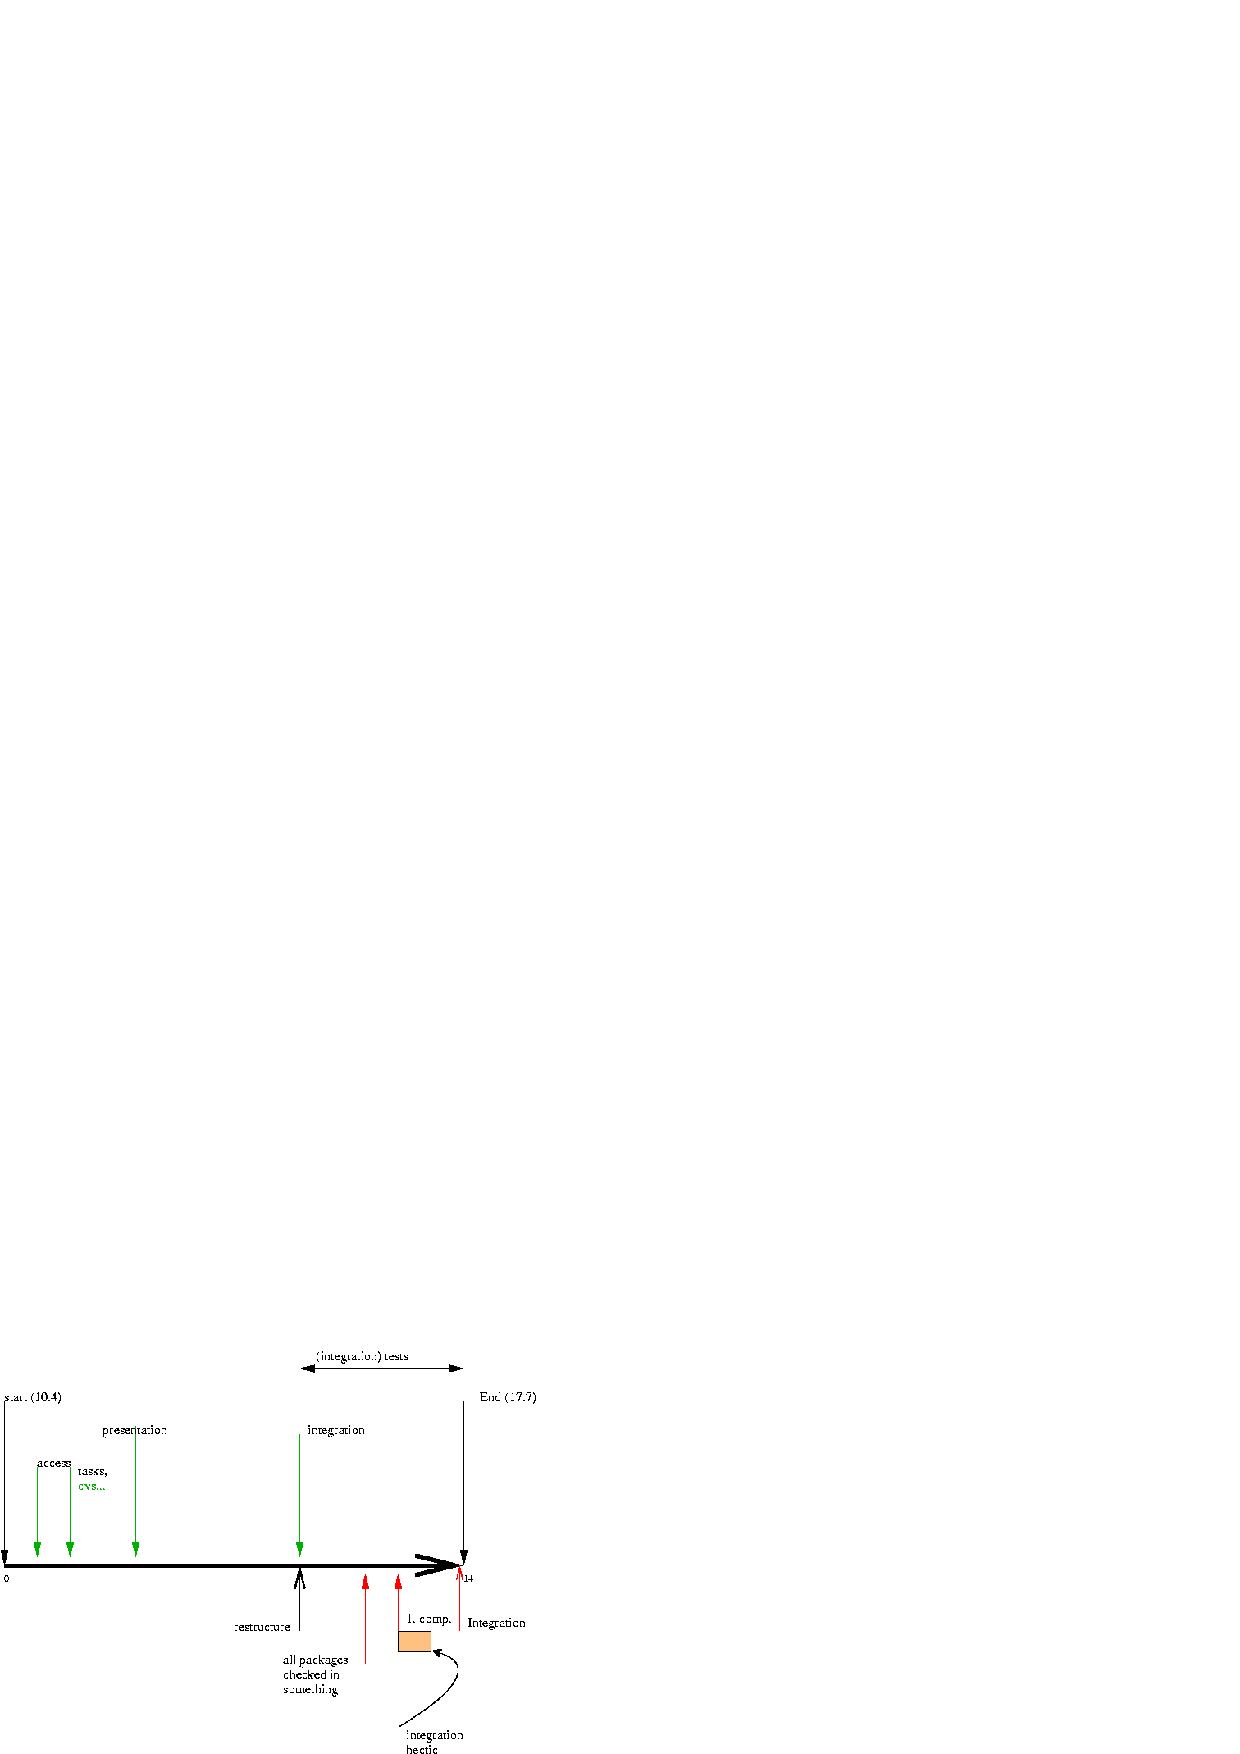
\includegraphics[clip=true,height=4.0cm]{timeline}}
  \item<3-> requirement specification is part of the task!
  \item<3-> success by
    \begin{itemize}
    \item<3-> initiative\footnote{Don't wait till someone else tells you what to
        do. Don't wait till the lazy group 12 does something.}
    \item<3-> openness, communication
    \item<4> (yes: and of course \importantxx{work} \ldots)
    \end{itemize}
  \end{itemize}
}


\frame{\frametitle{What we expect}
  \begin{itemize}
  \item active participation in \important{all} phases, in particular also
    the specification/setup phase
  \item active participation in the weekly meetings\footnote{take both parts
      \important{serious}! (the other parts, too, of course\ldots)}
  \item workable solution of the chosen task
  \item don't drop out in mid-flight
  \item timeliness
  \item during semester/end-of-semester: deliverables, demo and
    presentation(s)
  \end{itemize}
}
\section{Informal spec.}


\frame{\frametitle{\Coma}
  \begin{itemize}
  \item why this project?
  \item[$\Rightarrow$] simple reasons: 
    \begin{itemize}
    \item we (as \important{clients}) know vaguely what we ``want'',
    \item you (as \important{IT specialists}) probably don't exactly know what
      we want
    \end{itemize}
  \item conference manager:
  \item[]
    \shadowbox{
      \begin{minipage}[t]{9cm}
        A web-based tool to assist the distributed preparation,
        organi{z}ation, and processing of scientific conferences.
      \end{minipage}
    }
  \end{itemize}
}


\frame{\frametitle{Requirements}
  \begin{itemize}
  \item 4 main kinds of \important{customers}
    \begin{enumerate}
    \item  administrator: ``guru''
    \item authors: submit papers, wait for acceptance
    \item program commitee
      \begin{itemize}
      \item decides about acceptance/rejectance of contributions
      \end{itemize}
      \item chairman (1 or many): 
        \begin{itemize}
        \item boss/moderator of the program commitee
        \item taking final decision[
        \end{itemize}
    \end{enumerate}
  \item adaptability: product should be usable for many conferences
  \item ``maintainability'': product should be managable via the net
  \item ``\important{portability}'': should be deplayably/run with standard
  \item ``security'': it should not compromize the safety of the system
    software
  \end{itemize}
}

\frame{\frametitle{Possible tasks}
  \begin{itemize}
  \item data base(s)
  \item report generation, web page generation
  \item discussion tracking
  \item management of discussion status
  \item visualization of status
  \item algorithm for assignments
  \item interface for authors
  \item interface for maintainers
  \item interface for programm commitee
  \item [testing]
  \item [documentation/manual]
  \end{itemize}
}



\section{First timeline sketch}

\frame{\frametitle{Semster}
  \begin{itemize}
  \item fixed dates:
    \begin{enumerate}
    \item start: now
    \item end: end of semster: Friday, 11.\ February 2005
    \end{enumerate}
  \item[$\Rightarrow$] 15 tuesdays/ approx general 15 meeting during
    semester (i.e., without Christmas)
  \item at the end (as said)
    \begin{itemize}
    \item demo
    \end{itemize}
  \item wish: early \important{integration}\footnote{will be hard(er) this
      time.}
  \item wish: testing
  \end{itemize}
}

\frame{\frametitle{Today}
  \begin{itemize}
  \item supervisors
    \begin{itemize}
    \item introduction
    \item project intro and warm up (= now)
    \item CVS intro 
    \end{itemize}
  \item team
    \begin{itemize}
    \item personal introduction
    \item expertise of the team
    \item how many participants? 
    \item 4/8 hours?
    \item formation of \important{teams} of the \important{first phase}
    \end{itemize}
  \end{itemize}
}





\frame{\frametitle{first 2 weeks}

  \begin{itemize}
  \item get the ball rolling: $\Rightarrow$
  \item we need (at least) two teams\footnote{depending on how many we are}
    \begin{enumerate}
    \item taskforce ``\importantx{Spec}''
      \only<1>{
      \begin{itemize}
      \item explicit requirement definition of the requirement spec
      \item taking into consideration
        \begin{description}
        \item[-] manpower of the semester
        \item[-] \important{modularizability}, equal load
        \item[-] expertise of the members
        \end{description}
      \item sources
        \begin{description}
        \item[-] thinking
        \item[-] \important{discussion} with us\footnote{I.e., we need
            appointments.}
        \item[-] ``market analysis''
        \end{description}
      \item deliverables:
        \begin{description}
        \item[-] spec. document
        \item[-] presentation
        \end{description}
      \end{itemize}}
    \item taskforce ``\importantx{Tools}''
      \only<2>{
        \begin{itemize}
      \item selection of the tools/languages for the implementation
        \begin{description}
        \item[-] which database server (if any)
        \item[-] which language(s), which versions
        \item[-] \ldots
        \end{description}
      \item taking into consideration
        \begin{description}
        \item[-] manpower
        \item[-] local availability\footnote{we can of course install
            things}
        \item[-] expertise!
        \end{description}
      \item sources
        \begin{description}
        \item[-] discussion
        \item[-] ``market analysis''
        \end{description}
      \item deliverable
        \begin{description}
        \item[-] tools spec (versions)
        \item[-] presentation
        \item[-] expertise (i.e., being able to help the others)
        \item[-] availability of the tools
        \end{description}
      \end{itemize}}
  \item taskforce \importantx{Testing}
    \only<3>{
    \begin{itemize}
    \item make a test concept, deliverables: as the other task forces
    \end{itemize}}
  \end{enumerate}
\end{itemize}
}



\frame{\frametitle{Till/during next week}
  \begin{itemize}
  \item members
    \begin{itemize}
    \item get cvs \important{ready}(see handout)
    \item organize your \important{workplace}
    \item first appointments?
    \end{itemize}
  \item coordinators:
    \begin{itemize}
    \item make first informal spec ready
    \item make email adresses available
    \item finalize web-page
    \item organize further literature
    \end{itemize}
  \end{itemize}
}

\section{Misc}

\frame{\frametitle{Misc}
  \begin{itemize}
  \item current means of \important{communication}:
    \begin{itemize}
    \item email-addresses
    \item our web-page (hopefully always up-to date), contains
      \begin{enumerate}
      \item[-] results of discussions, handouts, links
      \item[-] decisions
      \item[-] current status  
      \item[] \ldots
      \end{enumerate}
    \end{itemize}
  \end{itemize}
}


%%% Local Variables: 
%%% mode: latex
%%% TeX-master: "main"
%%% End: 
